\begin{figure}[tb]
\centering
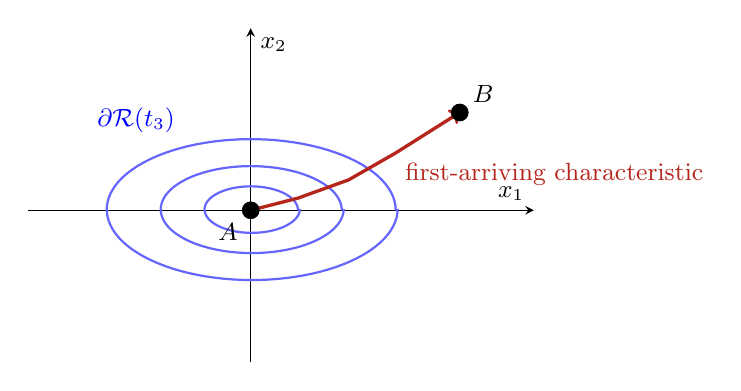
\begin{tikzpicture}[font=\small]
 \begin{axis}[width=.78\linewidth,height=.48\linewidth,axis equal image,
  axis lines=middle,xmin=-3.3,xmax=4.2,ymin=-2.25,ymax=2.7,ticks=none,xlabel={$x_1$},ylabel={$x_2$},clip=false]
  \foreach \a/\b/\c in {.7/.35/20,1.35/.65/35,2.15/1.05/55}{
   \addplot[blue!60,thick,domain=0:360,samples=100] ({.03*x/360+\a*cos(x)},{.02*x/360+\b*sin(x)});}
  \addplot[only marks,mark=*,black,mark size=3pt] coordinates {(0,0)(3.1,1.45)};
  \node[anchor=north east] at (axis cs:-.05,-.05) {$A$};
  \node[anchor=south west] at (axis cs:3.15,1.45) {$B$};
  \addplot[BrickRed,very thick,->] coordinates {(0,0)(.7,.18)(1.45,.45)(2.15,.85)(3.1,1.45)};
  \node[blue,anchor=south] at (axis cs:-1.7,1.0) {$\partial\mathcal R(t_3)$};
  \node[BrickRed,anchor=north west] at (axis cs:2.15,.85) {first-arriving characteristic};
 \end{axis}
\end{tikzpicture}
\caption{Reachability as an expanding wavefront.  Minimum time is the first
contact of the reachable set with the target; the optimal trajectory is a
characteristic of the arrival-time field.}
\label{fig:reachability-wavefront}
\end{figure}

